%%%%%%%%%%%%%%%%%%%%%%%%%%%%%%%%%%%%%%%%%
% Beamer Presentation
% LaTeX Template
% Version 1.0 (10/11/12)
%
% This template has been downloaded from:
% http://www.LaTeXTemplates.com
%
% License:
% CC BY-NC-SA 3.0 (http://creativecommons.org/licenses/by-nc-sa/3.0/)
%
% Modified by Nicholas J. Gotelli
% 9 January 2021
%%%%%%%%%%%%%%%%%%%%%%%%%%%%%%%%%%%%%%%
\documentclass[12pt]{beamer}\usepackage[]{graphicx}\usepackage[]{color}
% maxwidth is the original width if it is less than linewidth
% otherwise use linewidth (to make sure the graphics do not exceed the margin)
\makeatletter
\def\maxwidth{ %
  \ifdim\Gin@nat@width>\linewidth
    \linewidth
  \else
    \Gin@nat@width
  \fi
}
\makeatother

\definecolor{fgcolor}{rgb}{0.345, 0.345, 0.345}
\newcommand{\hlnum}[1]{\textcolor[rgb]{0.686,0.059,0.569}{#1}}%
\newcommand{\hlstr}[1]{\textcolor[rgb]{0.192,0.494,0.8}{#1}}%
\newcommand{\hlcom}[1]{\textcolor[rgb]{0.678,0.584,0.686}{\textit{#1}}}%
\newcommand{\hlopt}[1]{\textcolor[rgb]{0,0,0}{#1}}%
\newcommand{\hlstd}[1]{\textcolor[rgb]{0.345,0.345,0.345}{#1}}%
\newcommand{\hlkwa}[1]{\textcolor[rgb]{0.161,0.373,0.58}{\textbf{#1}}}%
\newcommand{\hlkwb}[1]{\textcolor[rgb]{0.69,0.353,0.396}{#1}}%
\newcommand{\hlkwc}[1]{\textcolor[rgb]{0.333,0.667,0.333}{#1}}%
\newcommand{\hlkwd}[1]{\textcolor[rgb]{0.737,0.353,0.396}{\textbf{#1}}}%
\let\hlipl\hlkwb

\usepackage{framed}
\makeatletter
\newenvironment{kframe}{%
 \def\at@end@of@kframe{}%
 \ifinner\ifhmode%
  \def\at@end@of@kframe{\end{minipage}}%
  \begin{minipage}{\columnwidth}%
 \fi\fi%
 \def\FrameCommand##1{\hskip\@totalleftmargin \hskip-\fboxsep
 \colorbox{shadecolor}{##1}\hskip-\fboxsep
     % There is no \\@totalrightmargin, so:
     \hskip-\linewidth \hskip-\@totalleftmargin \hskip\columnwidth}%
 \MakeFramed {\advance\hsize-\width
   \@totalleftmargin\z@ \linewidth\hsize
   \@setminipage}}%
 {\par\unskip\endMakeFramed%
 \at@end@of@kframe}
\makeatother

\definecolor{shadecolor}{rgb}{.97, .97, .97}
\definecolor{messagecolor}{rgb}{0, 0, 0}
\definecolor{warningcolor}{rgb}{1, 0, 1}
\definecolor{errorcolor}{rgb}{1, 0, 0}
\newenvironment{knitrout}{}{} % an empty environment to be redefined in TeX

\usepackage{alltt}
% only 10,11, or 12 pt fonts
% PACKAGES-----------------------------------
\usepackage{graphicx} % Allows including images
\usepackage{booktabs} % Allows the use of \toprule, \midrule and \bottomrule in tables

% THEMES AND COLORS-------------------------
\mode<presentation> {
\usefonttheme{professionalfonts}
% FONTTHEMES: default, structurebold, structuresmallcapsserif, structureitalicserif, serif, professionalfonts


\usetheme{Montpellier}
% THEMES: default, AnnArbor, Antibes, Bergen, Berkeley, Berlin, Boadilla, boxes, CambridgeUS, Copenhagen, Darmstadt, Dresden, Frankfurt, Goettingen, Hannover, Ilmenau, JuanLesPins, Luebeck, Madrid, Malmoe, Marburg, Montpellier, PaloAlto, Pittsburgh, Rochester, Singapore, Szeged, Warsaw

\usecolortheme{beetle}
%COLORTHEMES: default, albatross, beaver, beetle, crane, dolphin, dove, fly, lily, orchid, rose, seagull, seahorse, sidebartab, structure, whale, wolverine 

% DISPLAY OPTIONS--------------------------
\setbeamertemplate{footline} % To remove the footer line in all slides, uncomment this line

\setbeamertemplate{footline}[page number] % To replace the footer line in all slides with a simple slide count, uncomment this line

\setbeamertemplate{navigation symbols}{} % To remove the navigation symbols from the bottom of all slides, uncomment this line
}
% -----------------------------------------

% TITLE PAGE DATA--------------------------
\title[Short title]{Ethan Homework 4} % The short title appears at the bottom of every slide, the full title is only on the title page

\author{Ethan Dean} % Your name

\institute[UVM] % Your institution as it will appear on the bottom of every slide, may be shorthand to save space
{
University of Vermont \\ % Your institution for the title page
Department of Biology \\
Burlington, VT 05401 USA \\ 
\medskip
\textit{emdean@uvm.edu} % Your email address
}
\date{24 February 2021} % Date, can be changed to a custom date or \today
% -----------------------------------------

% BEGIN DOCUMENT---------------------------
\IfFileExists{upquote.sty}{\usepackage{upquote}}{}
\begin{document}

% OPTIONAL TITLE PAGE SLIDE----------------
\begin{frame}
\titlepage % Print the title page as the first slide
\end{frame}

% OPTIONAL TABLE OF CONTENTS SLIDE---------

\begin{frame}
\frametitle{Presentation Conents} % Table of contents slide, comment this block out to remove it
\tableofcontents % Throughout your presentation, if you choose to use \section{} and \subsection{} commands, these will automatically be printed on this slide as an overview of your presentation
\end{frame}

% OPTIONAL SECTION HEADERS-----------------
\section{Non-Writing} % Sections can be created in order to organize your presentation into discrete blocks; all sections and subsections are automatically printed in the table of contents as an overview of the talk

\subsection{List of Great Apes}
\subsection{Picture of a Great Apes}
% A subsection can be created just before a set of slides with a common theme to further break down your presentation into chunks

% SLIDE (BULLET POINTS)--------------------
\begin{frame}
\frametitle{Great Apes}
\begin{itemize}
\item Humans
\item Bonobo
\item Chimpanzee
\item Gorilla
\item Orangutan
\end{itemize}
\end{frame}

% SLIDE (SEQUENTIAL BULLET POINTS)---------
\begin{frame}
\frametitle{General Ape Hand Characteristics}
\begin{itemize}
\item<1-> Opposable Thumb
\item<2-> Sensitive tactile pads on digits
\item<3-> Flattened nails for digit protection
\end{itemize}
\end{frame}

% SLIDE (FIGURE)-----------------------------
\begin{frame}
\frametitle{Non-Human Great Apes}
% Uncomment the code on this slide to include your own image from the same directory as the template  file.
\begin{figure}
   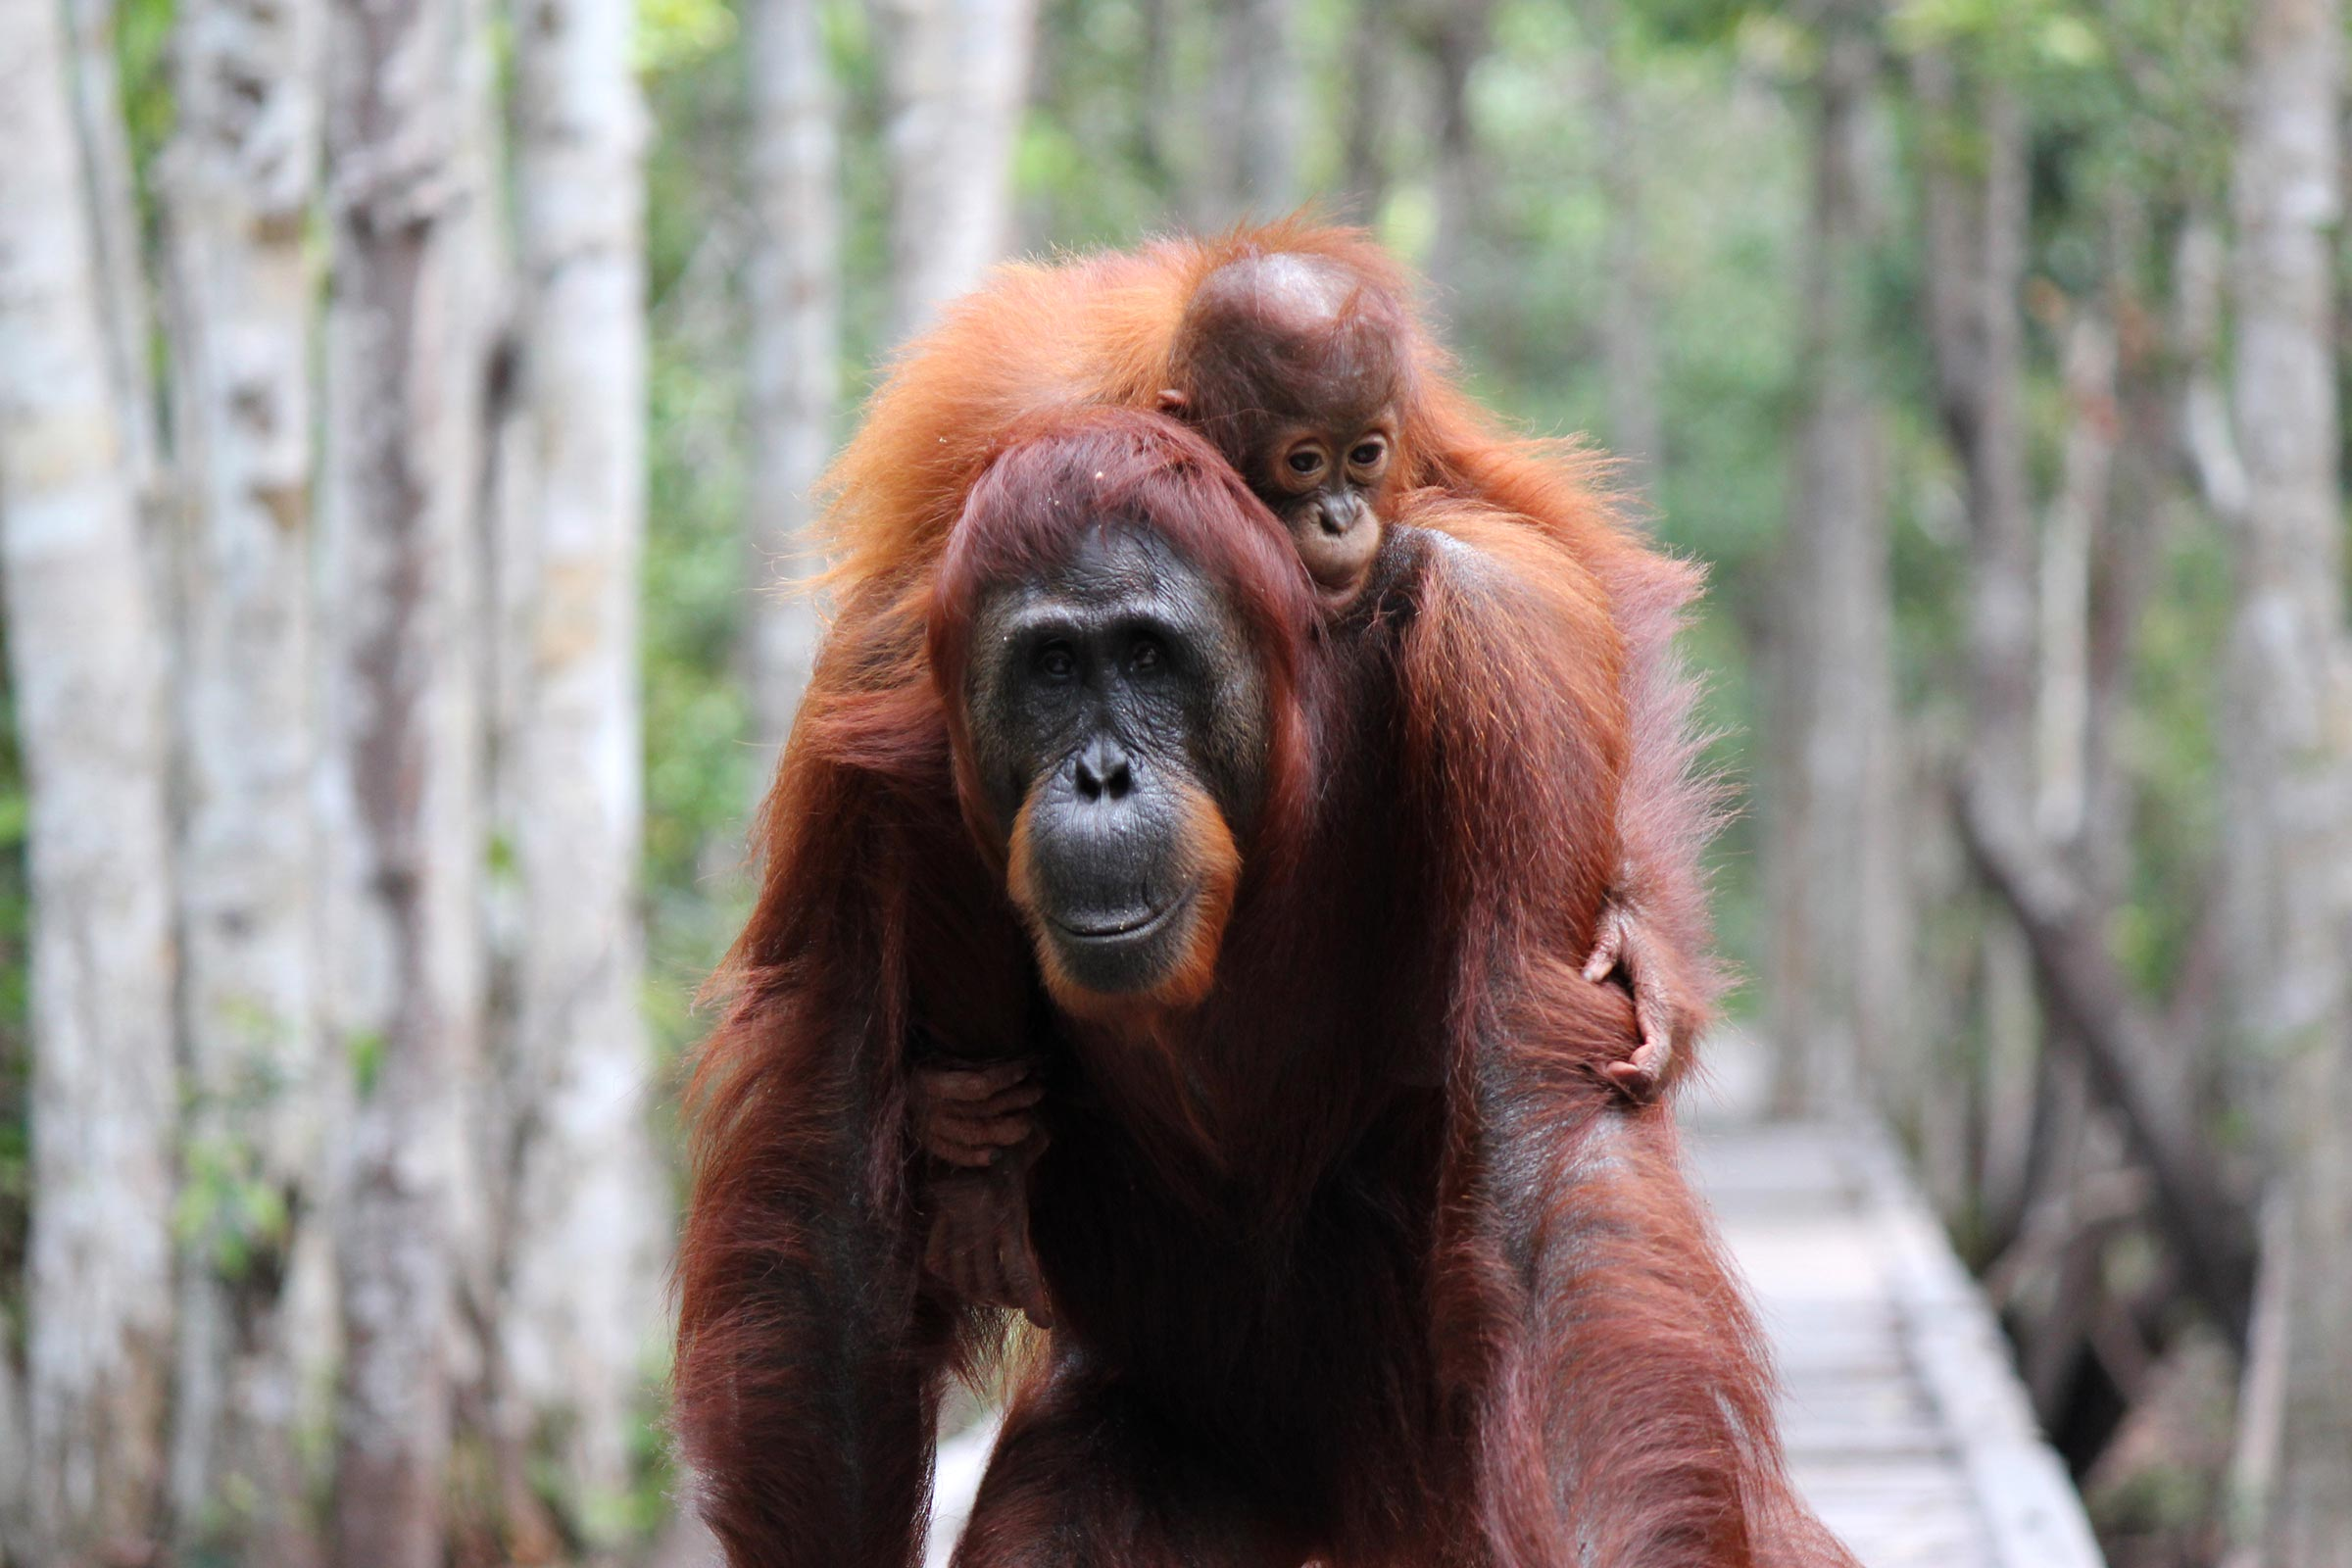
\includegraphics[width=0.475\linewidth]{orang.jpg}
   \hfill
   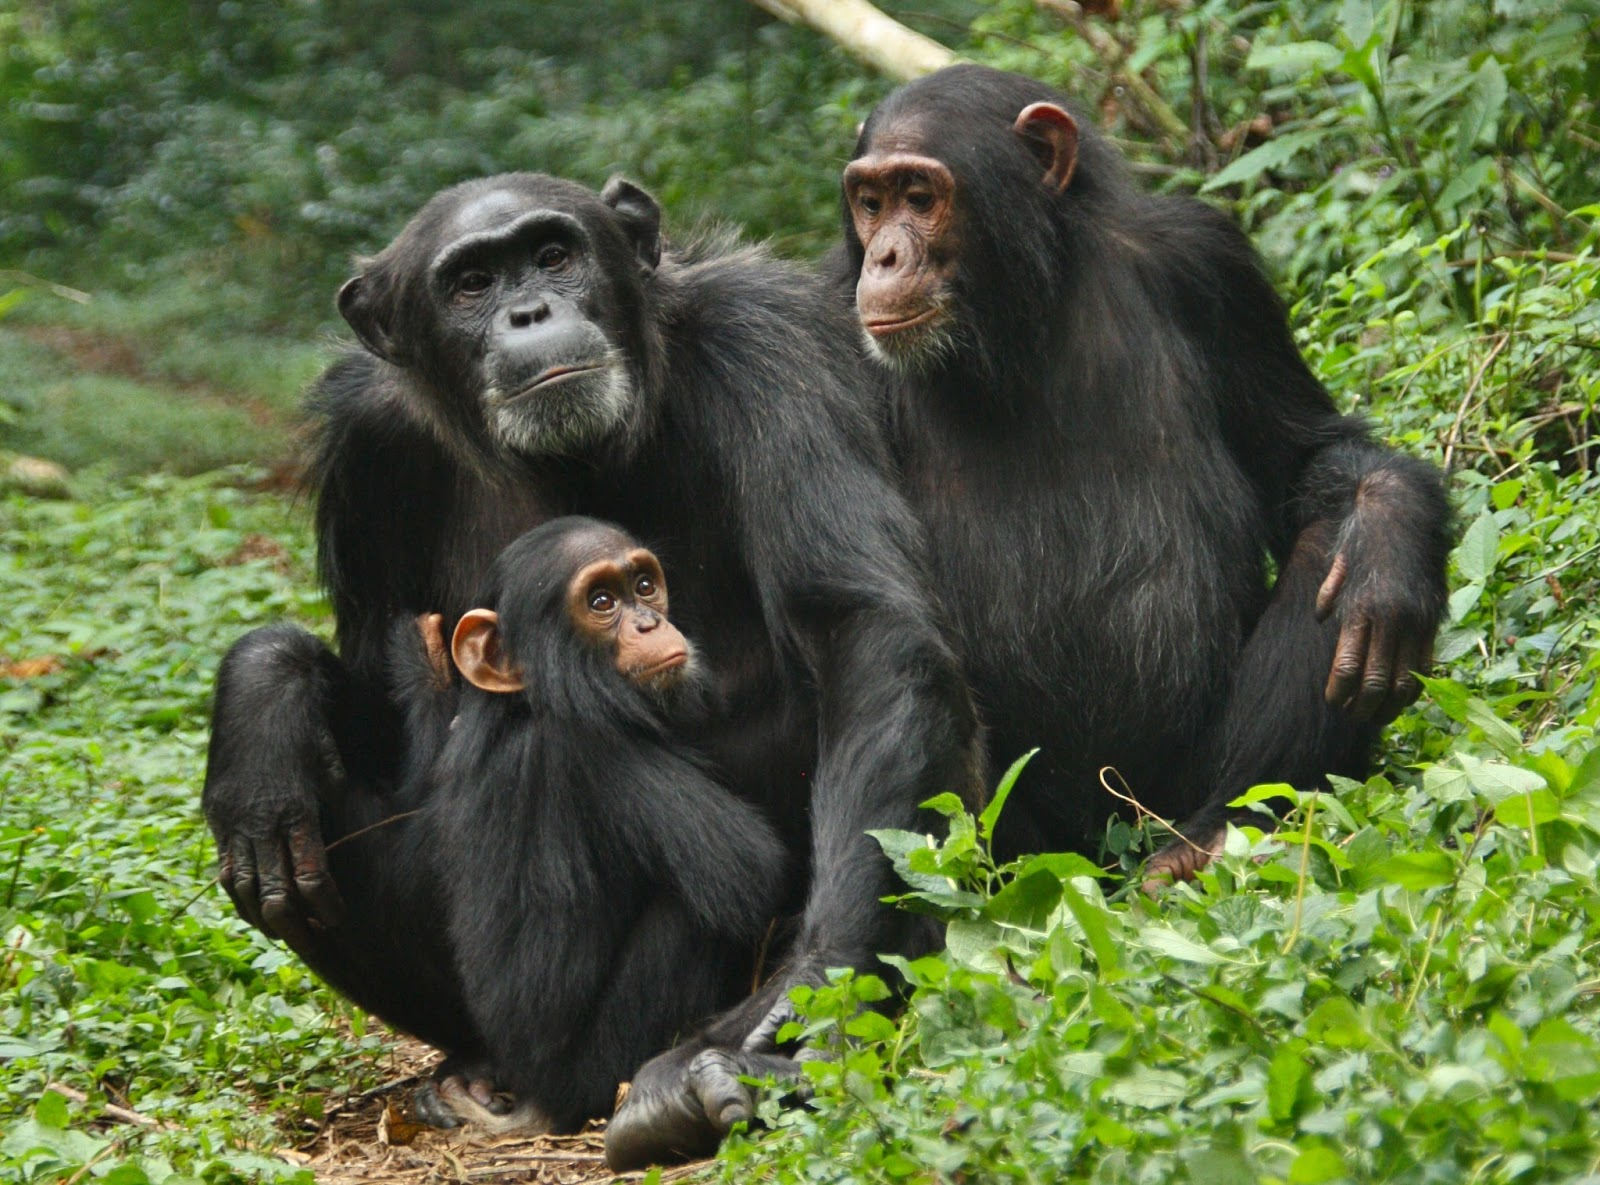
\includegraphics[width=0.475\linewidth]{chimp.jpg}
   \caption {Two picture of cute ape families} 
% use this format for absolute sizing
%\includegraphics[width=3cm, height=4cm]{filename.jpg}
\end{figure}
\end{frame}

% SLIDE (TABLE)----------------------------
\begin{frame}
\frametitle{Table}
\begin{table}
\begin{tabular}{l l l}
\toprule
\textbf{Apes} & \textbf{Relation} & \textbf{Habitat}\\
\midrule
Bonobo & Close & Democratic Republic of Congo \\
Mountain Gorilla & Middle & Democratic Republic of Congo \\
Sumatran Orangutan & Far & Indonesia (Sumatra) \\
\bottomrule
\end{tabular}
\caption{A comparison of different great ape types to their relation to humans and the area in which they are located}
\end{table}
\end{frame}

%------------------------------------------------
\section{Species Preservation}
%------------------------------------------------
% SLIDE (PARAGRAPHS OF TEXT)---------------
\begin{frame}
\frametitle{Great Apes}
Great apes are really amazing and share lots of similar characteristics with humans. However, they are all threatened in some manner so it is important to pay attention to the conservation status of our closest ancestors and make sure that we can keep their diversity around to appriciate.
\\~\\



\end{frame}

% SLIDE (BLOCKS OF HIGHLIGHTED TEXT)-------
%\begin{frame}
%\frametitle{Blocks of Highlighted Text}
%\begin{block}{Block 1}
%Lorem ipsum dolor sit amet, consectetur adipiscing elit. Integer lectus nisl, ultricies in feugiat rutrum, porttitor sit amet augue. Aliquam ut tortor mauris. Sed volutpat ante purus, quis accumsan dolor.
%\end{block}

%\begin{block}{Block 2}
%Pellentesque sed tellus purus. Class aptent taciti sociosqu ad litora torquent per conubia nostra, per inceptos himenaeos. Vestibulum quis magna at risus dictum tempor eu vitae velit.
%\end{block}

%\begin{block}{Block 3}
%Suspendisse tincidunt sagittis gravida. Curabitur condimentum, enim sed venenatis rutrum, ipsum neque consectetur orci, sed blandit justo nisi ac lacus.
%\end{block}
%\end{frame}

% SLIDE (EMBEDDED R CODE)------------------
%\begin{frame}[fragile]{Embedded R Code; \texttt{fragile} frame}
%\begin{block}



%\end{block}
%\end{frame}

% SLIDE (EMBEDDED R FIGURE)----------------
\begin{frame}[fragile]{Primate Fertility}%; %\texttt{fragile} frame}
\begin{block}

\begin{knitrout}
\definecolor{shadecolor}{rgb}{0.969, 0.969, 0.969}\color{fgcolor}

{\centering 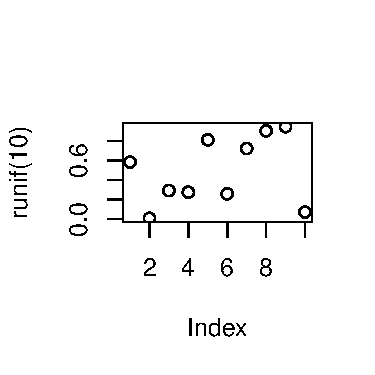
\includegraphics[width=\maxwidth]{figure/unnamed-chunk-2-1} 

}



\end{knitrout}

\end{block}
\end{frame}

% SLIDE (MULTIPLE COLUMNS)-----------------
%\begin{frame}
%\frametitle{Multiple Columns}
%\begin{columns}[c] % The "c" option specifies centered vertical alignment while the "t" option is used for top vertical alignment

%\column{.45\textwidth} % Left column and width
%\textbf{Heading}
%\begin{enumerate}
%\item Statement
%\item Explanation
%\item Example
%\end{enumerate}

%\column{.5\textwidth} % Right column and width
%Lorem ipsum dolor sit amet, consectetur adipiscing elit. Integer lectus nisl, ultricies in feugiat rutrum, porttitor sit amet augue. Aliquam ut tortor mauris. Sed volutpat ante purus, quis accumsan dolor.

%\end{columns}
%\end{frame}


% SLIDE (THEOREM)----------------------------
%\begin{frame}
%\frametitle{Theorem}
%\begin{theorem}[Mass--energy equivalence]
%$E = mc^2$
%\end{theorem}
%\end{frame}

% SLIDE (VERBATIM)---------------------------
%\begin{frame}[fragile] % Need to use the fragile option when verbatim is used in the slide
%\frametitle{Verbatim}
%\begin{example}[Theorem Slide Code]
%\begin{verbatim}
%\begin{frame}
%\frametitle{Theorem}
%\begin{theorem}[Mass--energy equivalence]
%$E = mc^2$
%\end{theorem}
%\end{frame}\end{verbatim}
%\end{example}
%\end{frame}

% SLIDE (FINAL SLIDE)------------------------
\begin{frame}
\Huge{\centerline{FIN}}
\end{frame}

%------------------------------------------------
\end{document}
